\documentclass[11pt]{article}


\usepackage[a4paper,
            mag=1000, includefoot,
            left=3cm, right=1.5cm, top=2cm, bottom=2cm, headsep=1cm, footskip=1cm]{geometry}

% \linespread{1.5}
% \allowdisplaybreaks[4]o

%\documentclass[11pt]{article}
\usepackage[utf8]{inputenc}
%\usepackage[english]{babel}
\usepackage{graphicx}
%\usepackage{caption}
\usepackage[table,xcdraw]{xcolor}
\usepackage{epigraph}
\usepackage{float}

%\usepackage{amssymb}
%\usepackage{amsmath}
%%

\usepackage{latexsym,amssymb,amsthm}
\usepackage{amsfonts}
%\usepackage[T2A]{fontenc}
\usepackage{amsmath}
\usepackage{url}

\usepackage{indentfirst}

%\usepackage{refcheck} 


 % \voffset -24.5mm
 % \hoffset -5mm
 % \textwidth 173mm
 % \textheight 240mm
 % \oddsidemargin=0mm \evensidemargin=0mm

\numberwithin{equation}{section}
\newtheorem{theorem}{Theorem}[section]
\newtheorem{lemma}{Lemma}[section]
\newtheorem{proposition}{Proposition}[section]
\theoremstyle{definition}
%\theoremstyle{remark}
\newtheorem{remark}{Note}[section]
\newtheorem{corollary}{Corollary}[section]
\newtheorem{example}{Example}[section]
\newtheorem{definition}{Definition}[section]

\setcounter{tocdepth}{2}

\newcommand{\cov}{\mathrm {cov}}
% \newcommand{\Pr}{\mathrm {Pr}}

\usepackage{color}

\title{A Gentle Introduction to Compressed Sensing}
\author{Andrey V. Bzikadze}

\begin{document}

\maketitle
\epigraph{The \textbf{data deluge} refers to the situation where the volume of new data being generated is overwhelming the capacity of institutions to manage it and researchers to make use of it.}

\section{Introduction}
In the last decade the humanity has come to the point when it produces much more information than it can store and analyse.
There is a huge exposion in the variety of sensors and their dimensionality in many areas: video, audio, scientific, medical research.
Because of that we face the problem of \textbf{data deluge} and naturally come to the necessity of compressing data.

\begin{figure}[H]
    \begin{center}
        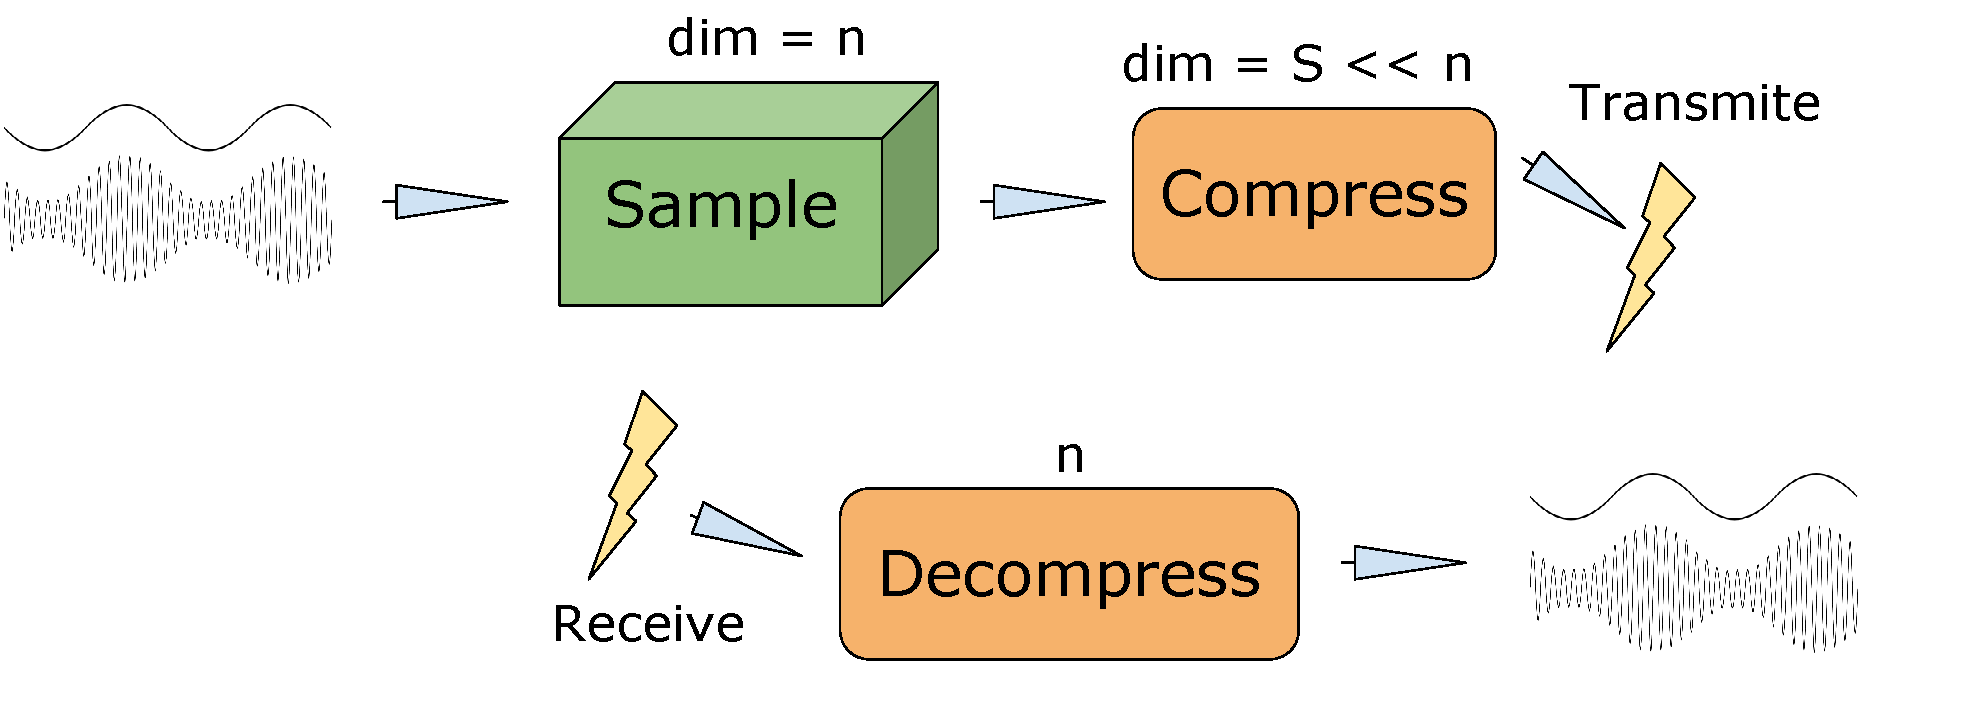
\includegraphics[width=.75\textwidth]{figures/CS_sample_compress_paradigm.pdf}
    \end{center}
    \caption{
        \label{fig:CSSampleCompressParadigm}
        ``Sample-Then-Compress Paradigm''.
        Sample could be a digital camera, a microphone, \ldots. Compression strategy is signal-dependent.
    }
\end{figure}
Let us consider the so-called ``Sample-Then-Compress Paradigm'' (Fig~\ref{fig:CSSampleCompressParadigm}).
We want to transmit a signal (it could be continuous), but are unable to do it with a whole signal.
Thus, we sample it $n$ times.
The transmission channel we use reduces the ``dimension'' of the sampled signal to $S \ll n$.
Afterwards, the received compressed signal is decompressed to previous dimension which is equal to $n$.
In this scenario $S$ is signal-nature-specific.
First, with $S \ll n$ the process seems to be somewhat wasteful.
Secondly, every sampling (measurement) could be exorbitant.
Thus, we want to reduce $n$ as much as it is possible.


The idea of Compressed Sensing is that the signal at Fig.~\ref{fig:CSSampleCompressParadigm} that we would like to transmit/acquire is actually sparse (or ``approximately sparse'') signal in a certain ``basis''.
Suppose that this signal is an $m$-dimensional vector.
Then we want to find a linear basis in $\mathbb R^m$ for this vector to be $S$-sparse.
The challenge of the problem is that we do not observe the signal explicitly (in any basis).
We can make sampling (measurements) that are a certain transformation of the signal (for example, linear).
Speaking non-formally, our aim is to reconstruct the signal making as few measurements as possible (to reduce $n$ at Fig.~\ref{fig:CSSampleCompressParadigm}).
Without the assumption of the existence of the basis in which the original signal is sparse the problem would have a trivial solution: we would generally need to make as many measurements as is the dimension of a signal.

Generally speaking there are 2 distinct problems:
\begin{itemize}
    \item to find a basis in which the signal is sparse (or approx sparse),
    \item to exactly / approximately reconstruct the signal observing a minimum possible number of measurements.
\end{itemize}
There are theoretical results yielding the minimum number of required measurements needed to produce the original signal given a specific measurement strategy.

In these notes we will not consider the problem of finding the basis in which the signal can be decomposed in a sparse manner.
We will only limit ourselves to a very small example given in the section \ref{sec:motivation} that demonstrates that this assumption is feasible.
Our main concern will be the second problem: to find and quantify the minimal possible number of measurements to reconstruct the original signal.

\section{An example of Compressed Sensing sparsity}
\label{sec:motivation}
The main idea of the Compressed Sensing is that a signal vector of our interest is a \textbf{sparse} vector when represented in \textbf{some basis}.
Technically speaking it could be not sparsity in a strict sense (when many components are zeros), but the approximately sparsity (when many components are close to zero).
There are lots of non-formal examples demonstrating this idea, however, many of them are very difficult to formalize.
We will stick to a very simple example that makes a connection with the time series theory.

Let us consider a time series $x = \{x_n\}_{n=1}^N$.
The time series $x$ itself is very rarely a sparse vector, i.e. one would not rely on the assumption that $x_n = 0$ for many $n$-s.
However, what could be assumed is that the periodogram has only a few peaks.
Indeed, let us suppose for all $n \in 1:N$
$$ x_n = \sum_{i=1}^S \sin\left(2 \pi w_i \frac{n}{N}\right), $$
where $w_i \in [0, 0.5]$ and $w_i \neq w_j$ for $i \neq j$.
We will suppose that the length $N$ is multiple of the period of $x$.
Then the periodogram will have peaks only at $w_i$.
In this sense the \textbf{Fourier basis} is the basis in which $x$ is $S$-\textbf{sparse}.

If with previous assumptions 
$$ x_n = \sum_{i=1}^k \sin\left(2 \pi w_i \frac{n}{N}\right) + \varepsilon_n, $$
for all $n \in 1:N$
where $\varepsilon_n$ is some noise with considerably low variance and zero mean.
Then the periodogram aside possessing peaks at $w_i$ will have small coefficients at the points.
In this sense the \textbf{Fourier basis} is the basis in which $x$ is \textbf{approximately} $S$-\textbf{sparse}.

\section{Problem Statement}
From now on we will only consider the problem of exact or approximate reconstruction of the signal observing a minimum possible number of measurements.

We fix $m \in \mathbb N$ and will denote the signal $\beta^*$ and will suppose that $\beta^* \in \mathbb R^m$.
We suppose that $\beta^*$ is (strictly) $S$-sparse (has only $S$ non-zero components).
This will be denoted as $\|\beta^*\|_0 = S$.
The $S$ itself is latent (not observed).
We also fix the set of design transformation matrices $\mathbf X_n \in \mathcal M_{n \times m}(\mathbb R)$ for all $n \in \mathbb N$.
The ``measurements'' are denoted $y_n \in \mathbb R^n$ for all $n \in \mathbb N$.
The formal connection between $\beta^*$ and $y_n$ is made through the matrix $\mathbf X_n$ for all $n \in \mathbb N$ and will be explicitly stated.

Let us note one more time that we are aware of $X_n$ for all $n$ and observe $y_n$, but do not observe $\beta^*$ and want to find it with the smallest $n$ possible.

\subsection{Noiseless case}
Let us suppose that $y_n = X_n \beta^*$ for all $n \in \mathbb N$.
The problem is to obtain $\beta^*$ as the solution of the linear system $y_n = \mathbf X_n \beta$ (the variable $\beta$).
The illustration can be seen at Fig.~\ref{fig:NoiseLessProblemStatement}.
\begin{figure}[H]
    \begin{center}
        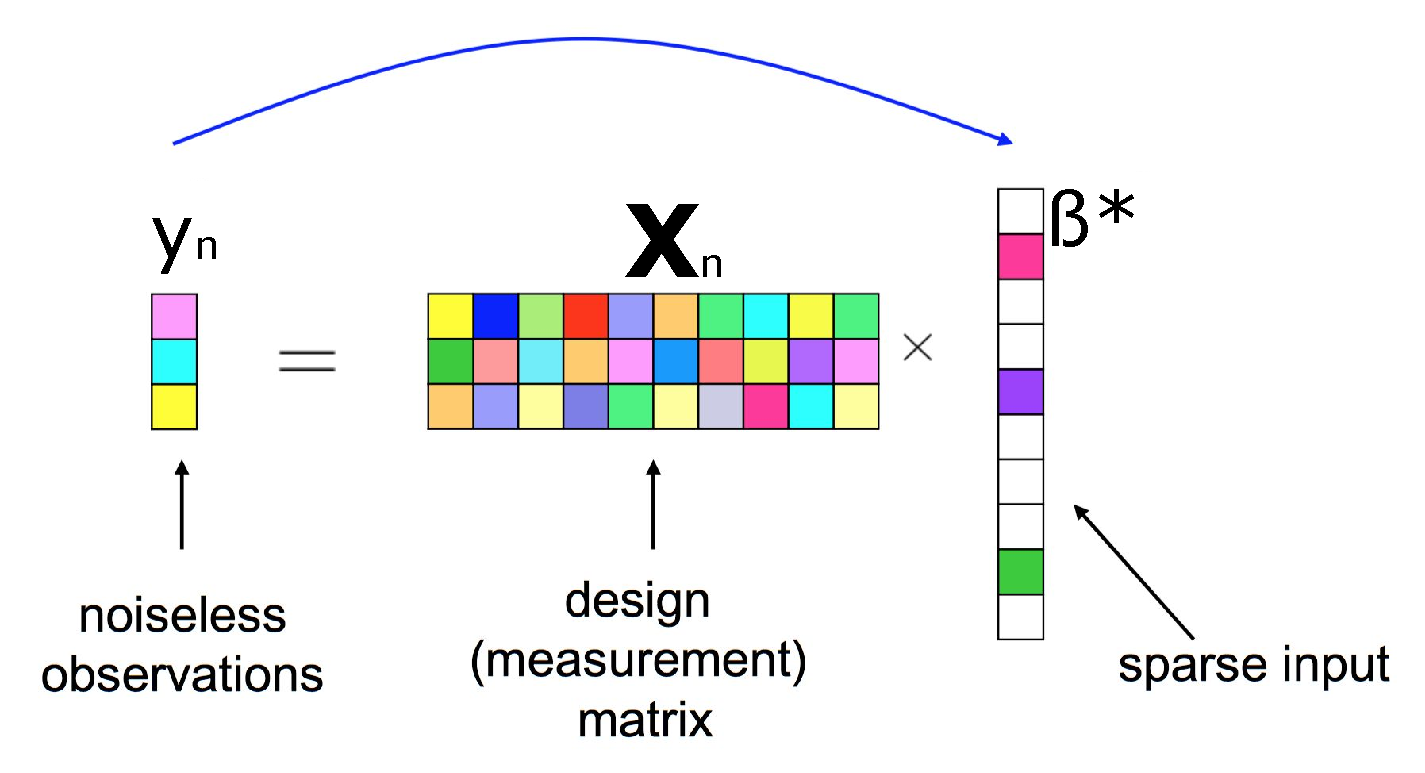
\includegraphics[width=.75\textwidth]{figures/problem_statement_2.pdf}
    \end{center}
    \caption{
        \label{fig:NoiseLessProblemStatement}
        Noiseless problem statement.
    }
\end{figure}

For each $n$ we present the following estimator
\begin{gather}
    \label{eq:noiselessBeta}
    \hat \beta_n = \arg \min_{\beta: y_n = \mathbf X_n \beta} \|\beta\|_1.
\end{gather}

The choice of $n$ such that $\hat \beta = \beta^*$ is heavily influenced by $S$ and $\mathbf X_n$.
We will now consider an example of the family $\{\mathbf X_n\}_{n \geqslant 1}$.

\begin{definition}
    \label{def:rip}
    A matrix $\mathbf A \in \mathcal M_{n, m}(\mathbb R)$ is said to satisfy the \textbf{restricted isometry property} of order $S$ with constant $\delta_S$ for $\delta_S \in (0, 1)$ if
    $$ (1 - \delta_S) \|x\|_2^2 \leqslant \|\mathbf A x\|_2^2 \leqslant (1 + \delta_S) \|x\|_2^2 $$
    for all $S$-sparse $x \in \mathbb R^m$.
    
    Notation: $\mathbf A \in \textrm{RIP}(S, \delta_S)$.
\end{definition}

\begin{theorem}
    Let $\mathbf X_n \in \mathcal M_{n, m} (\mathbb R)$ be $\textrm{RIP}(S, \delta)$ where $S \leq m / 2$ and $\delta \in (0, 1)$. Then for
    $$ n \geqslant C_\delta S \log(m / S), $$
    where $C_\delta < 1$ is a constant and depends only on $\delta$:
    $$ \hat \beta_n = \beta. $$
\end{theorem}
Proof can be found in Theorem 3.5: \url{mdav.ece.gatech.edu/publications/phdthesis-2010.pdf}.

It is an NP-problem to check whether the matrix satisfies RIP.
However, it is easy to simulate a matrix that satisfies RIP with a high probability.

\begin{theorem}
    Fix $\delta \in (0, 1)$.
    Let $\mathbf X_n \in \mathcal M_{n, m} (\mathbb R)$ be a random matrix whose components are independent and have $\mathcal N(0, 1/n^2)$ distribution.
    If for some $C_1 > 0$
    $$ n \geqslant C_1 \log(m / S), $$
    then 
    $$ \mathbb P(\mathbf X_n \in \textrm{RIP}(S, \delta)) \geq 1 - 2 e^{-C_2 n}, $$
    where $C_2 = \delta^2/2C_1 - \ln (42 e / \delta) / C_1$.
\end{theorem}
Proof can be found in Theorem 4.3: \url{mdav.ece.gatech.edu/publications/phdthesis-2010.pdf}.

Let us note that the RIP quality is not the only condition that allows to formulate such results.
There are plenty of them, see Section 3.1.3: \url{https://sites.google.com/site/igorcarron2/cs}

\subsection{Noisy case}
Let us suppose that $y_n = X_n \beta^* + \varepsilon_n$ for all $n \in \mathbb N$, where $\varepsilon_n$ is the noise.
The conditions on it with be formalized further.
The problem is to obtain $\beta^*$ as an approximate solution to the linear system $y_n \approx \mathbf X_n \beta$ (the variable $\beta$).
The illustration can be seen at Fig.~\ref{fig:NoisyProblemStatement}.
\begin{figure}[H]
    \begin{center}
        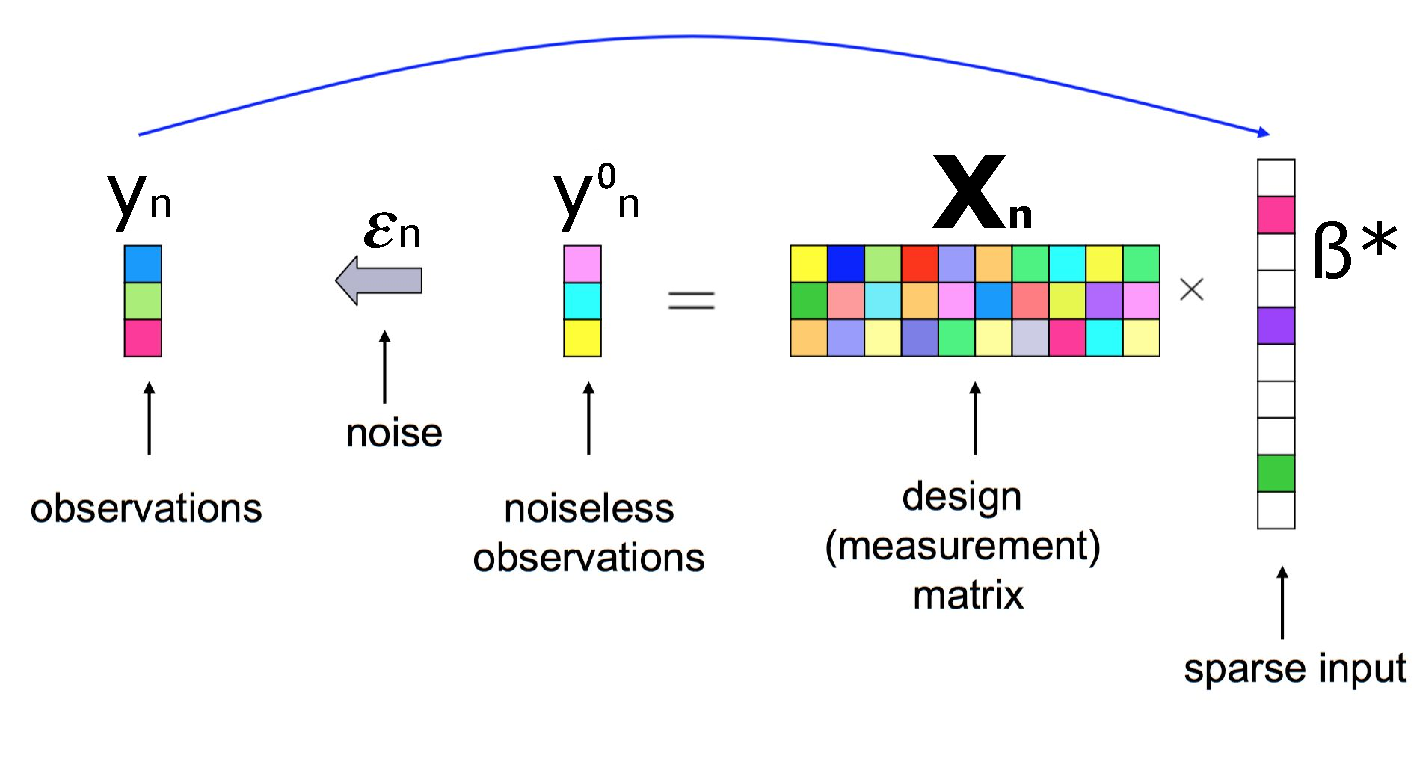
\includegraphics[width=.75\textwidth]{figures/problem_statement_3_noisy.pdf}
    \end{center}
    \caption{
        \label{fig:NoisyProblemStatement}
        Noisy problem statement.
    }
\end{figure}

For each $n$ and accuracy $\delta > 0$ we present the following estimator
\begin{gather*}
    \hat \beta_n(\delta) = \arg \min_{\beta: \|y_n - \mathbf X_n \beta\|_2^2 \leqslant \delta} \|\beta\|_1.
\end{gather*}

The choice of $n$ such that $\hat \beta \approx \beta^*$ is heavily influenced by $S$ and $\mathbf X_n$.
The results similar to the noiseless case hold here for RIP matrices.

Let us consider the following elaboration on the optimization problem:
$$ \min_{\beta: \|y_n - \mathbf X_n \beta\|_2^2 \leqslant \delta} \|\beta\|_1 $$
is equivalent to LASSO:
$$ \min_{\beta: \|\beta\|_1 \leqslant t} \|y_n - \mathbf X_n \beta\|_2^2 $$
for a certain $t$.
Thus, we can apply the numerical procedures for LASSO problem (LARS).

\section{Random Fourier projections (Candes et al., 2006)}

This section is devoted to a special choice of the matrices $\mathbf X_n$.
Formally we change the notation.
Let $\mathcal F$ be the Fourier basis matrix in $\mathbb R^m$, $\mathbb T = 1:m$ --- a set of all time points when the measurements could be conducted, $\Omega \subset \mathbb T$ --- when the measurements are conducted.

Instead of \eqref{eq:noiselessBeta} consider
\begin{gather}
    \hat \beta_n = \arg \min_{\substack{\beta: (\mathcal F \beta^*)_t = (\mathcal F \beta)_t \\ t \in \Omega}} \|\beta\|_1.
\end{gather}
The noisy problem is reformulated analogously.

The fundamental result is the following:
\begin{theorem}
    Let $\beta^* \in \mathbb C^m$, $\|\beta^*\|_0 = S$. Let $\Omega \subset \mathbb T$ be a uniformly selected set of a fixed size $n_\Omega$.
    Fix $B > 0$ --- accuracy.
    If
    $$ n_\Omega \geq C(B) n \ln m, $$
    where $C(B) \asymp 23(B + 1)$ then
    $$ \mathbb P(\hat \beta_n = \beta^*) \geq 1 - \mathcal O(m^{-B}). $$
\end{theorem}

\begin{remark}
    $\Omega \subset \mathbb T$ --- a uniformly selected set of a fixed size $n_\Omega$ --- is very difficult to simulate.
    However, we can change this condition to the set of Bernoulli trials:
    $$ \Omega: \mathbb P(j \in \Omega) = \tau $$
    and the theorem changes only slightly.
\end{remark}

\section{The Recovery Theorem for arbitrary bases}

\begin{definition}
    Let $\Phi = \{\phi_i\}$ and $\Psi = \{\psi_j\}$ be the bases in $\mathbb R^m$.
    Then the \textbf{coherence} of orthonormal bases $\Phi$ and $\Psi$.
    $$ \mu(\Phi, \Psi) = \sqrt{m} \max_{i, j} |(\phi_i, \psi_j)|. $$
\end{definition}

\begin{remark}
    Two facts about the coherence:
    \begin{enumerate}
        \item $ 1 \leq \mu(\Phi, \Psi) \leq \sqrt m $.
        \item $\mu(\mathcal F, \mathcal F^{-1}) = 1$.
    \end{enumerate}
\end{remark}

\begin{theorem}[Candes and Romberg, 2007]
    Fix $\delta > 0$, $\beta^* \in \mathbb R^m$.
    Choose $\Omega$ uniformly (of a fixed size).

    Consider the solution to the following convex optimization problem:
    $$ \hat \beta = \arg \min_\beta \|\beta\|_1: (\beta^*, \phi_k) = (\phi_k, \Psi \beta), k \in \Omega. $$
    
    If
    $$ |\Omega| \ge C \mu^2(\Phi, \Psi) \|\beta^*\|_0 \ln \frac{m}{\delta} $$
    then
    $$ \mathbb P(\hat \beta = \beta^*) \ge 1 - \delta. $$
\end{theorem}

\begin{remark}
    The following results about the noisy problem are formulated for RIP matrices and will be out of scope.
\end{remark}

\end{document}
